\subsection{Drivetrain}\label{Drivetrain}

The drive train on the given belt vehicle is what translates the torque $\tau_m$ given by the motor into the actual movement of the vehicle. The model of this system part shows the relation between the applied rotational force (or torque) $\tau_m$ and the speed of the belts. It is still considered that the vehicle's tajectory follows a straight line.\\\\
%
Different iterations of this model can be made to get more acuraccy. The first of these iterations should give an overview of how the system reacts to a given torque input. 

\subsubsection{Black Box Model}\label{BlackBoxModel}
To get a rough approximation of how the drive train works, a black box model is used. There is a small gear $G_m$ on the motor shaft, which is in contact with another actual gear $G_2$. The imaginary gear $G_d$ represents the differential and the gears and shafts of the drivetrain from (and including) this second gear $G_2$ to the gears that drive the belt, see \figref{fig:DrivetrainMechanicalModel}.

\begin{figure}[H]
	\centering
	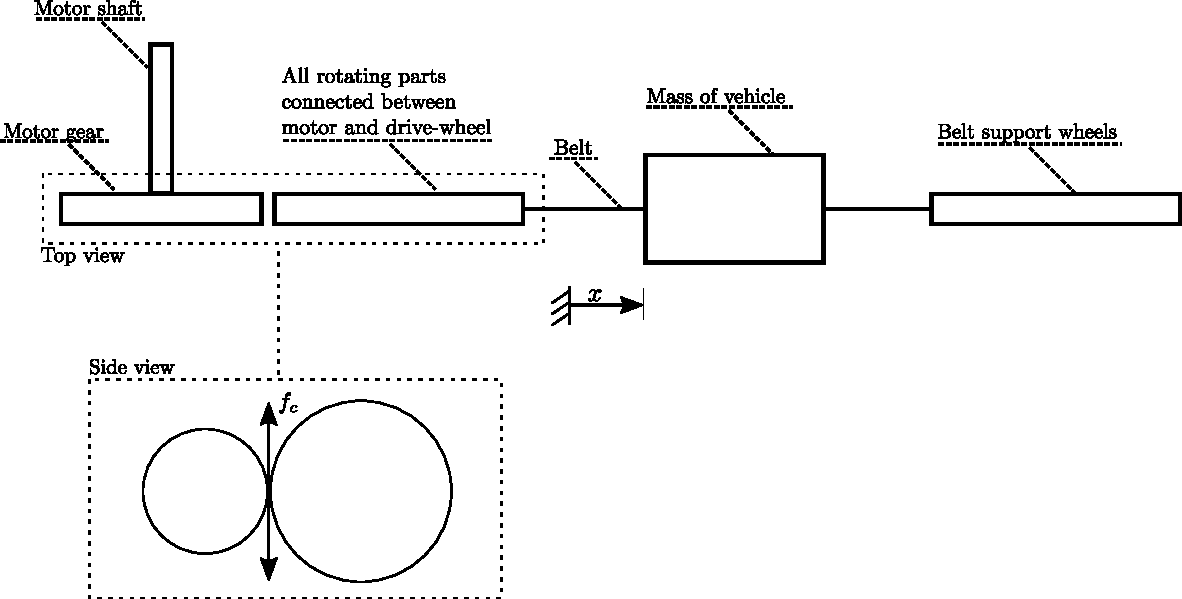
\includegraphics[scale=0.8]{figures/mechanicalDrawing.pdf}
	\caption{A simple mechanical diagram of the vehicle drivetrain}
	\label{fig:DrivetrainMechanicalModel}
\end{figure}
\todo{Add notations to the diagram and create free body diagrams of belt and black box parts}

\begin{figure}[H]
	\centering
	%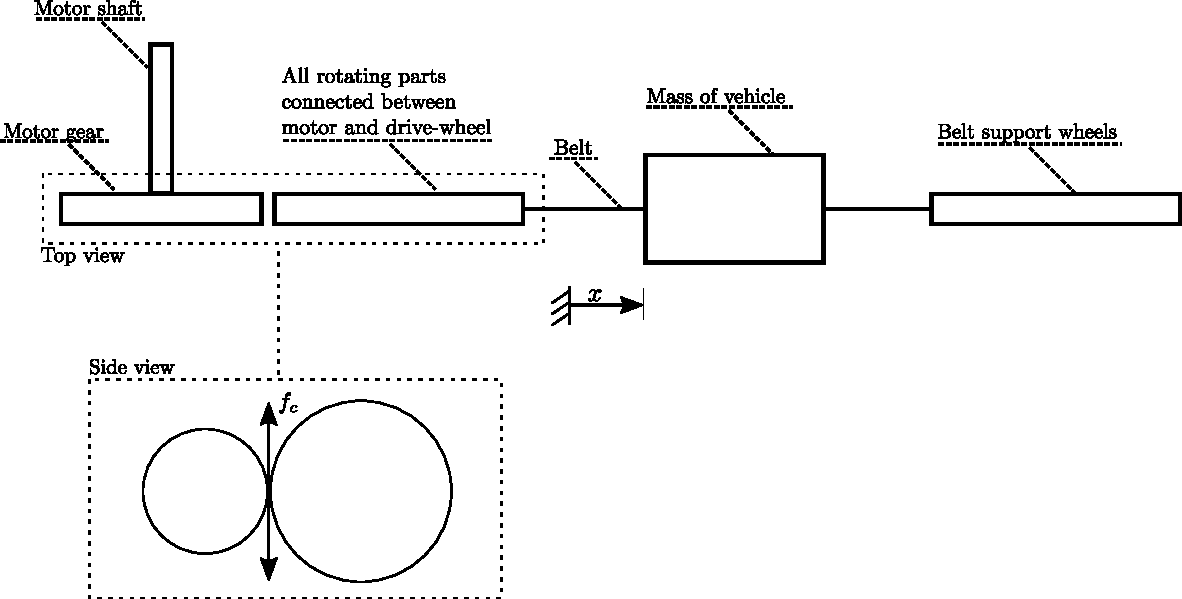
\includegraphics[scale=0.8]{figures/mechanicalDrawing.pdf}
	\caption{A free body diagram of the motor gear and `black-box' gear}
	\label{fig:GearsFreeBodyDiagram}
\end{figure}

From \figref{fig:GearsFreeBodyDiagram} and Newton's second law appplied to rotational systems, we can extract the equation :


\begin{flalign}\centering
J_m \cdot \dot{\omega}_m(t) = \tau_m(t) - B_m \cdot \omega_m(t) - N_m \cdot f_c(t) 
\label{eq:mechanicalmodel}
\end{flalign}
\hspace{6mm} Where\\
\begin{tabular}{p{1cm}ll}
& $J_m$ 			      & is the motor's inertia [$kg*m^2$] \\
& $\omega_m$        & is the angular velocity of the motor [$rad*s^{-1}$] \\
& $\dot{\omega}_m$ 	& is the angular acceleration of the motor [$rad*s^{-2}$] \\
& $\tau_m$ 		     	& is the torque delivered by the motor [$N$] \\
& $B_m$             & is the coefficient of the friction happening inside the motor [$N*s*rad^{-1}$] \\
& $N_m$             & is the number of teeth of the motor gear $G_m$ [$number\ of\ teeths$] \\
& $f_c$             & is the coefficient of the contact force between $G_m$ and $G_d$ [$N*number\ of\ teeths^{-1}$]

\end{tabular}
\todo{Discuss about units (use siunitx?) and equations conventions inside the report}

\begin{figure}[H]
	\centering
	%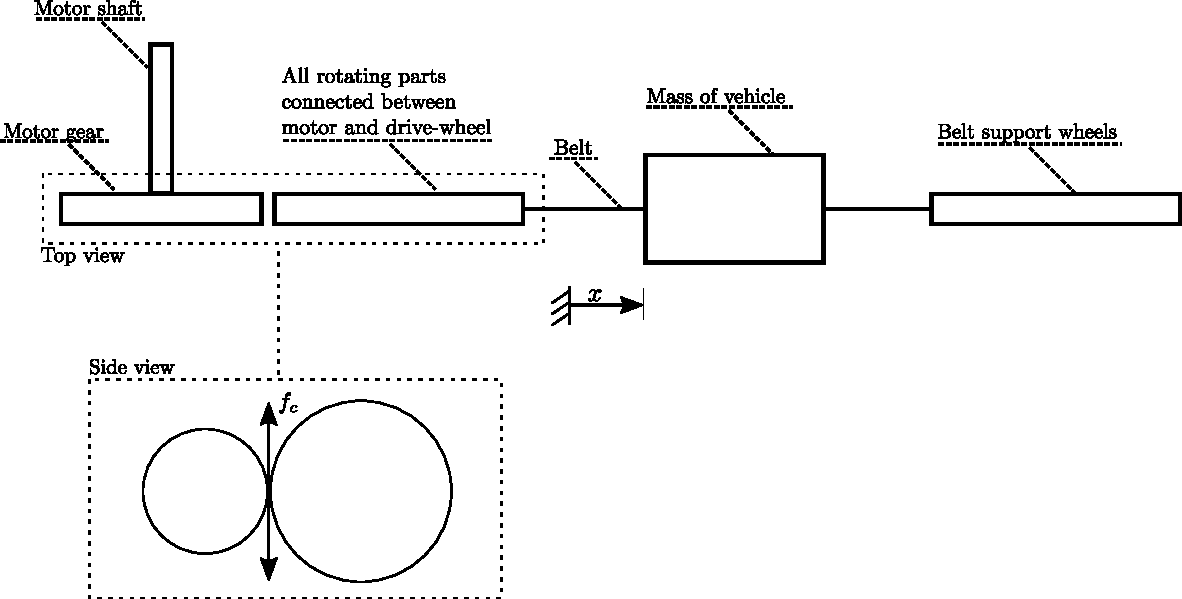
\includegraphics[scale=0.8]{figures/mechanicalDrawing.pdf}
	\caption{A mechanical diagram of the belt part}
	\label{fig:BeltFreeBodyDiagram}
\end{figure}

\begin{figure}[H]
	\centering
	%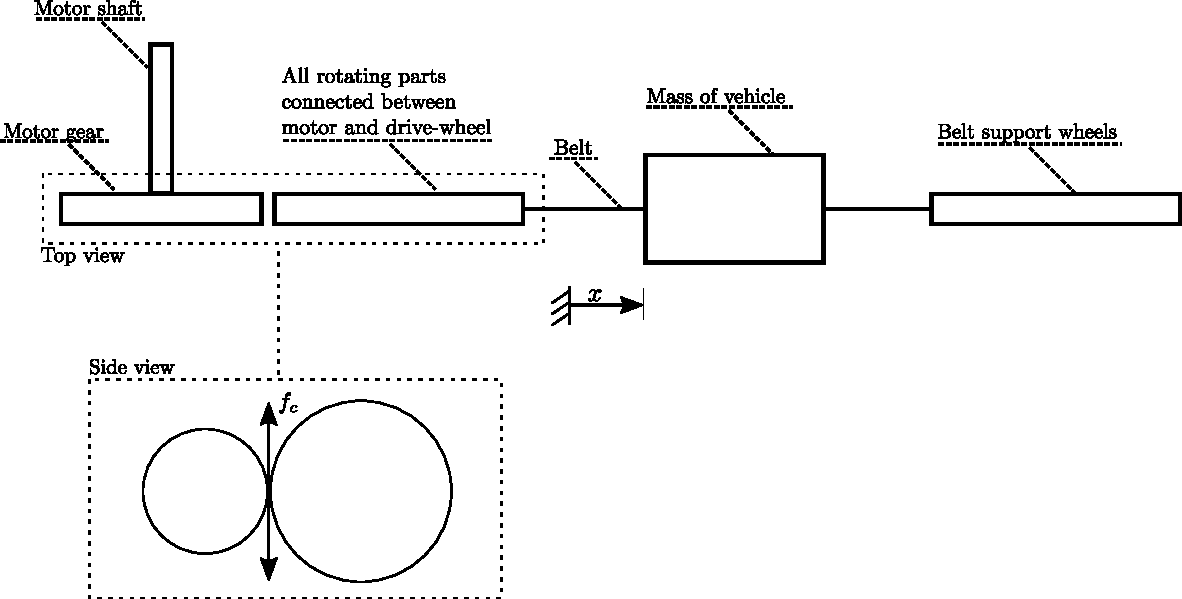
\includegraphics[scale=0.8]{figures/mechanicalDrawing.pdf}
	\caption{A free body diagram of the belt driven mass}
	\label{fig:BeltFreeBodyDiagram}
\end{figure}